% -*- mode: fundamental -*-

% ****************************************************************

\chapter{The core functions for RISC-V execution}

\markboth{Ch \arabic{chapter}: Core functions (DRAFT)}{\copyrightnotice}

\setcounter{page}{1}
% \renewcommand{\thepage}{\arabic{page}}
\renewcommand{\thepage}{\arabic{chapter}-\arabic{page}}

\label{ch_core_functions}

% ****************************************************************

\section{Introduction}

In this chapter we discuss the core functions of
Figure~\ref{Fig_Simple_Instr_Exec_w_structs}, which we repeat here for
convenience (all the \verb|struct| declarations can be found in the
file: \verb|src_Common/Inter_Stage.bsv|).
\begin{figure}[htbp]
  \centerline{\includegraphics[width=6in,angle=0]{ch030_RISCV_Design_Space/Figures/Fig_Instr_Exec_w_structs}}
  \caption{\label{Fig_Fetch_function_Simple_Instr_Exec}Simple interpretation of RISC-V instructions (same as Fig.~\ref{Fig_Instr_Exec}, with arrows annotated with {\tt struct} types)}
\end{figure}

% ****************************************************************

\section{RISC-V: The Fetch function}

\label{Sec_Fetch_function}

The Fetch function \emph{per se} is fairly simple, even trivial.  Its
input is the current value of the program counter (PC), which is used
as the address in a memory-request to IMem.  It has two outputs,

\begin{tightlist}

 \item A \emph{memory request} to memory, to read an instruction.  We
   have already seen the definitition of the \verb|Mem_Req| struct in
   the previous chapter.

 \item Some additional information ``\verb|F_to_D|'' passed on to the
 Decode step.

\end{tightlist}

The ``\verb|F_to_D|'' struct has only one interesting field, the PC:

\begin{Verbatim}[frame=single, numbers=left]
typedef struct {
   Bit #(XLEN) pc;
} F_to_D
deriving (Bits, FShow);
\end{Verbatim}

\index{BSV!struct@{\tt struct}!Single-field structs}

\vspace*{2ex}

NOTE:
\fbox{\small
\begin{minipage}{5in}

{\bf BSV: single-field structs}

It might seem like overkill to define a struct for just one field like
the PC (why not just pass the PC?), but it has the following advantages:

\begin{itemize}

  \item It becomes easy to add more fields later, should we need to do
    so.  In particular, for Fife we will need to add some
    branch-prediction information.  We may also wish to add temporary
    fields that aid in debugging.

  \item Stronger type-checking: each new struct type is distinct from
    all other types in a BSV program.  Thus, the type-checker will
    catch any error where we may inadvertantly pass some unrelated and
    irrelevant XLEN-wide value in place of an {\tt F\_to\_D} struct.

  \item There is \emph{no} runtime cost: an {\tt F\_to\_D} value
    occupies the same XLEN bits as the {\tt pc} field by itself.

\end{itemize}

\end{minipage}}

\vspace*{2ex}

\index{BSV!struct!Nested}

To pass both results of \verb|fn_F|, we simply use a \emph{nested}
struct, {\ie} a struct containing the two component structs:

\begin{Verbatim}[frame=single, numbers=left]
typedef struct {
   F_to_D   to_D;        // info to Decode step
   Mem_Req  mem_req;     // requst info to memory
} Result_F
deriving (Bits, FShow);
\end{Verbatim}

Finally, as mentioned earlier, the function \verb|fn_F| is almost
trivial:

\begin{Verbatim}[frame=single, numbers=left]
function Result_F fn_F (Bit #(XLEN)  pc)
   let y = Result_F {to_D: F_to_D {pc: pc},
                     mem_req: Mem_Req {req_type: MEM_LOAD,
                                       size:     MEM_4B,
                                       addr:     pc,
                                       data :    ?}};
   return y;
endfunction
\end{Verbatim}

% ================================================================

\hdivider

% ----------------
\Exercise

Write a testbench for \verb|fn_F()|, apply it to a number of 32-bit
values (PC values) and print the results using \verb|$display| and
\verb|fshow|, and visually check that the \verb|F_to_D| and
\verb|Mem_Req| outputs look correct.

\Endexercise

% ****************************************************************

\section{RISC-V: The Decode function}

\label{Sec_Combo_Decode}

\index{fn\_D@{\tt fn\_D}!Decode function}
\index{Decode function!fn\_D@{\tt fn\_D}}

The core function for the Decode step is called \verb|fn_D|.  It's
arguments are an \verb|F_to_D| struct from the Fetch step and a
\verb|Mem_Rsp| memory response struct from memory.  It's output struct
type , \verb|D_to_RR|, was described in
Section~\ref{Sec_struct_D_to_RR}.  The code for \verb|fn_D| is mostly
a big if-then-else that analyses the incoming instruction and produces
some summary information:

\begin{Verbatim}[frame=single, numbers=left]
function D_to_RR
         fn_D (F_to_D  x_F_to_D, Mem_Rsp  rsp_IMem);

   Bit #(32) instr = truncate (rsp_IMem.data);
   Bit #(5)  rd    = instr_rd (instr);

   let fallthru_pc = x_F_to_D.pc + 4;

   // Baseline info to next stage
   let y = D_to_RR {pc:           x_F_to_D.pc,

                    exception:    False,
                    cause:        ?,

                    // not-exception
                    fallthru_pc: fallthru_pc,
                    instr:       instr,
                    opclass:     ?,
                    has_rs1:     False,
                    has_rs2:     False,
                    has_rd:      False,
                    writes_mem:  False,
                    imm:         0};

   if (rsp_IMem.rsp_type == MEM_RSP_MISALIGNED) begin
      y.exception = True;
      y.cause     = cause_INSTRUCTION_ADDRESS_MISALIGNED;
   end
   else if (rsp_IMem.rsp_type == MEM_RSP_ERR) begin
      y.exception = True;
      y.cause     = cause_INSTRUCTION_ACCESS_FAULT;
   end
   else if (is_legal_LUI (instr) || is_legal_AUIPC (instr)) begin
      y.opclass = OPCLASS_IALU;
      y.has_rd  = non_zero_rd;
      y.imm     = zeroExtend (instr_imm_U (instr));
   end
   else if (is_legal_BRANCH (instr)) begin
      y.opclass = OPCLASS_CONTROL;
      y.has_rs1 = True;
      y.has_rs2 = True;
      y.imm     = zeroExtend (instr_imm_B (instr));
   end
   else if (is_legal_JAL (instr)) begin
      y.opclass = OPCLASS_CONTROL;
      y.has_rd  = non_zero_rd;
      y.imm     = zeroExtend (instr_imm_J (instr));
   end
   else if (is_legal_JALR (instr)) begin
      y.opclass = OPCLASS_CONTROL;
      y.has_rs1 = True;
      y.has_rd  = non_zero_rd;
      y.imm     = zeroExtend (instr_imm_I (instr));
   end
   else if (is_legal_LOAD (instr)) begin
      y.opclass = OPCLASS_MEM;
      y.has_rs1 = True;
      y.has_rd  = non_zero_rd;
      y.imm     = zeroExtend (instr_imm_I (instr));
   end
   else if (is_legal_STORE (instr)) begin
      y.opclass    = OPCLASS_MEM;
      y.has_rs1    = True;
      y.has_rs2    = True;
      y.writes_mem = True;
      y.imm        = zeroExtend (instr_imm_S (instr));
   end
   else if (is_legal_OP_IMM (instr)) begin
      y.opclass = OPCLASS_IALU;
      y.has_rs1 = True;
      y.has_rd  = non_zero_rd;
      y.imm     = zeroExtend (instr_imm_I (instr));
   end
   else if (is_legal_OP (instr)) begin
      y.opclass = OPCLASS_IALU;
      y.has_rs1 = True;
      y.has_rs2 = True;
      y.has_rd  = non_zero_rd;
   end
   else if (is_legal_ECALL (instr) || is_legal_EBREAK (instr)) begin
      y.opclass = OPCLASS_SYSTEM;
   end
   else if (is_legal_FENCE (instr) || is_legal_FENCE_I (instr)) begin
      y.opclass = OPCLASS_FENCE;
      y.has_rs1 = True;
      y.has_rd  = non_zero_rd;
   end
   else begin
      y.exception = True;
      y.cause     = cause_ILLEGAL_INSTRUCTION;
   end

   return y;
endfunction
\end{Verbatim}

In line 4, we extract the instruction from the \verb|Mem_Rsp| memory
response from the Fetch operation, and in line 5 we extract the
\verb|rd| (``destination register'') field from the instruction.

\index{truncate@{\tt truncate}!operation to shrink bit-width}

In line 4, the \verb|truncate| operation is used to shrink the
bit-vector width of \verb|rsp_IMem.data| to the bit-vector width of
\verb|instr| (32-bits).  But why is this shrinkage needed?  After all,
in the declaration of the \verb|Mem_Rsp| type, the \verb|data| field
is declared to have type \verb|Bit#(XLEN)| which is synonymous with
\verb|Bit#(32)|.  The reason is that we've written the code to be
ready for re-use in the future with RV64, when \verb|XLEN| will be
defined as 64.  The \verb|truncate| operation is polymorphic,
accepting arguments of any bitwidth wider than the required output.
Here, when the argument is 32-bits wide, it does nothing (is a no-op);
but for RV64, when the argument is 64-bits wide, it performs the
shrinkage to 32 bits.  Note, \verb|truncate| keeps least-significant
bits and drops most-significant bits.

In line 7 we compute the fall-through PC, PC+4 (with the caveat that
if we want to support the ``C'' RISC-V ISA extension (``Compressed''
instructions), it may be PC+2, which information can be gleaned from
the instruction encoding).

In lines 10-23 we create a baseline \verb|D_to_RR| value which we will
selectively modify in the if-then-elses below.

In lines 25-32 we first handle the sitation where the Fetch operation
to memory itself returned an error.  We mark the \verb|exception|
field True and fill in the appropriate \verb|cause|.

The rest of the code is a series of if-then-else clauses. Each clause
identifies one class of instruction and updates the \verb|opclass|
field correspondingly.  The repertoire of instructions that we
consider are the forty instructions listed in the ``RV32I Base
Instruction Set'' table of ``Table 24.2: Instruction listing for
RISC-V'' of the Unprivileged Spec~\cite{RISCV_Unpriv_2019_12_13}.

Each if-then-else clause also fills in the \verb|has_rs1|,
\verb|has_rs2| and \verb|has_rd| fields, as appropriate, for each
class of instruction.  We also decode each kind of ``immediate'' field
and fill in the \verb|imm| field.

The final ``else'' clause is evaluated if the instruction does not
match one of the forty RV32I instructions.  In this case we set the
\verb|exception| and \verb|cause| fields to indicate an illegal
instruction.

Note the use of functions \verb|instr_imm_I()|, \verb|instr_imm_S()|,
\verb|instr_imm_B()|, \verb|instr_imm_U()| and \verb|instr_imm_J()|,
which extract the ``immediate'' field from a 32-bit instruction.  For
the different classes of instruction (I, S, B, U, J), the immediates
are coded differently, and have different widths (see the schemata at
the top of the RV32I page in ``Table 24.2: Instruction listing for
RISC-V'' of the Unprivileged Spec~\cite{RISCV_Unpriv_2019_12_13}).
These functions decode the bits and zero-extend them to XLEN bits (the
width of \verb|d_to_rr.imm|).  Later, in the ``execute'' code for each
instruction, we will pick out the relevant bits out of the XLEN bits,
and zero-extend or sign-extend them as needed for the particular
instruction.

An exercise below suggests that you write the code for these
\verb|instr_imm_X| functions; it's good practice for the BSV beginner!

Observe that the entire \verb|fn_D()| function is just a (large)
combinational circuit---it is an acyclic composition of smaller
combinational circuits, many of which we've seen earlier.  The whole
\verb|fn_D()| function can be visualized as a box with incoming wires
corresponding to \verb|F_to_D| and \verb|Mem_Rsp|, outgoing wires
corresponding to \verb|D_to_RR|, and filled with logic gates that
compute each output wire as a function of the input wires.

% ================================================================

\hdivider

% ----------------
\Exercise

Write the functions \verb|instr_imm_I()|, \verb|instr_imm_S()|,
\verb|instr_imm_B()|, \verb|instr_imm_U()| and \verb|instr_imm_J()|.

% ----------------
\Exercise

Write a testbench for \verb|fn_D()|, apply it to a number of PC and
instruction values.  For each input PC value, construct an
\verb|F_to_D| struct around it.  For each input instruction, construct
a \verb|Mem_Rsp| struct around it, some with memory errors, some
without.  Apply \verb|fn_D| to such pairs.  Print the results results
using \verb|$display| and \verb|fshow|, and visually check that the
\verb|D_to_RR| outputs look correct.

\Endexercise

% ****************************************************************

\section{RISC-V: The Register-Read function}

\label{Sec_fn_RR}

\index{fn\_RR@{\tt fn\_RR}!Register-read function}
\index{Register-read function!fn\_RR@{\tt fn\_RR}}

% ****************************************************************

\section{RISC-V: The Execute Control function}

\label{Sec_fn_Control}

\index{fn\_Control@{\tt fn\_Control}!Execute Control function}
\index{Execute Control function!fn\_Control@{\tt fn\_Control}}

% ****************************************************************

\section{RISC-V: The Execute Integer ALU function}

\label{Sec_fn_IALU}

\index{fn\_IALU@{\tt fn\_IALU}!Execute IALU function}
\index{Execute IALU function!fn\_IALU@{\tt fn\_IALU}}

% ****************************************************************

\section{RISC-V: The Execute DMem function}

\label{Sec_fn_DMem}

\index{fn\_DMem@{\tt fn\_DMem}!Execute DMem function}
\index{Execute DMem function!fn\_DMem@{\tt fn\_DMem}}

% ****************************************************************

\section{RISC-V: The Retire function}

\label{Sec_fn_Retire}

\index{fn\_Retire@{\tt fn\_Retire}!Retire function}
\index{Retire function!fn\_Retire@{\tt fn\_Retire}}

% ****************************************************************
